%=========================================================================
% sec-xpc
%=========================================================================

\section{Explicit-Parallel-Call Architectures}
\label{sec-xpc}

In software, XPC applications use a highly productive parallel
programming library allowing users to cleanly \emph{expose} varying forms
of amorphous data parallelism as fine-grain parallel tasks. Tasks are
exposed to hardware as parallel function calls via a unifying XPC ISA. In
addition, a software runtime facilitates adaptive \emph{scheduling} of
these tasks on the available XPC tiles. Dynamic task scheduling can be
accelerated in hardware with dedicated structures for storing and
distributing tasks. Finally, parallel tasks can be \emph{executed} on
either a traditional multicore or a combination of heterogeneous XPC
tiles specialized for exploiting varying forms of amorphous data
parallelism.

\subsection{Exposing Fine-Grain Parallel Tasks}

To expose opportunities for fine-grain parallel tasks, a productive
parallel programming libary and special XPC ISA extensions will be
provided.

The goal of the XPC programming library is to allow users to focus on an
algorithm-centric instead of a platform-centric approach to writing
applications. This in contrast to many traditional programming frameworks
that are low-level and specific to a single processor style (e.g., POSIX
threads). The programming library offers multiple parallel primitives to
make encoding amorphous data parallelism easier. Figure~\ref{fig-xpc-api}
shows a preliminary sketch of how the XPC library could be used to
parallelize two example applications. The \TT{spawn} primitive is used to
recursively generate tasks in a divide-and-conquer approach similar to
Intel Cilk++~\cite{cilk-spec2010}. The \TT{parallel\_for} primitive is
used to parallelize iterations/tasks of a loop. The \TT{atomic\_for}
primitive is similar to \TT{parallel\_for} except that it guarantees
iterations/tasks are processed atomically with respect to other
iterations/tasks. The \TT{speculative\_for} primitive extends
\TT{atomic\_for} by splitting tasks into reserve and commit phases where
tasks reserve any elements they need to access, and only commit if their
reservations were successful. Both \TT{atomic\_for} and
\TT{speculative\_for} have built-in conflict resolution for workloads
with tasks that need to modify the underlying data structure
concurrently. We take advantage of modern C++11 lambda functions to
achieve a clean and convenient method for defining tasks. Variables used
in the lambda are automatically captured by reference, and the API
handles passing in the appropriate index as an argument to the function.

\begin{figure}
  \begin{minipage}[b]{0.44\tw}
    %=========================================================================
% fig-xpc-api.tex
%=========================================================================

%\begin{figure*}

  \cbxsetfontsize{8pt}
  \begin{subfigure}{\tw}
  \begin{Verbatim}[gobble=6]
    void bfs( Node nodes[] ) {
      xpc::spawn( start, func = [&] (int idx) {

        Node my_node = node[idx];

        for ( i = 0; i < my_node.num_neigh; i++ ) {

          Node neighbor = my_node.neighbors[idx];

          if ( my_node.dist + 1 < neighbor.dist ) {
            neighbor.dist = my_node.dist + 1;
            xpc::spawn( neighbor.idx, func );
          }
        }});}
  \end{Verbatim}
  \end{subfigure}

  \caption{\BF{Example Code Using XPC Programming API --} Preliminary
    ideas for how the XPC programming API could be used to parallelize
    amorphous data parallel applications. The \TT{spawn} primitive is
    used to parallelize the breadth-first search application using a
    divide-and-conquer algorithm.}
  \label{fig-xpc-api}

%\end{figure*}

  \end{minipage}%
  \hfill%
  \begin{minipage}[b]{0.54\tw}
    %=========================================================================
% fig-xpc-isa.tex
%=========================================================================

%\begin{figure}

  \centering
  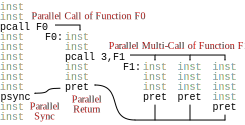
\includegraphics[width=\tw]{xpc-isa.svg.pdf}

  \caption{\textbf{XPC Instruction Set Overview --} Parallel calls and
    parallel multi-calls (\TT{pcall}) encode opportunities for parallel
    execution, which the architecture may (or may not) choose to exploit.
    Parallel synchronization points (\TT{psync}) require all child
    parallel calls to complete before continuing. All parallel returns
    (\TT{pret}) are implicitly synchronization points.}

  \label{fig-xpc-isa}

%\end{figure}


  \end{minipage}
\end{figure}

The tasks generated by these primitives can be managed purely in software
using cactus stacks~\cite{frigo-hyperobjects-spaa2009}, which associates
each task with a local view of the software stack. However, the XPC ISA
can be used to explicitly expose fine-grain parallel tasks to hardware as
parallel function calls. The XPC ISA extends a traditional RISC ISA with
three new instructions: a parallel function call instruction
(\TT{pcall}), a parallel function return instruction (\TT{pret}), and a
parallel synchronization instruction (\TT{psync}). A parallel function
call enables the software to inform the hardware that it is acceptable to
execute the callee in parallel with the caller, but critically, parallel
execution is \emph{not required}. A serial execution of any \TT{pcall}
should always be an acceptable execution. As illustrated in
Figure~\ref{fig-xpc-isa}, \TT{pcall}s can be nested to arbitrary depths,
and recursive \TT{pcall}s are also allowed. A \TT{psync} acts as a
synchronization point (i.e., barrier) and waits for all child \TT{pcall}s
to finish execution. For a serial execution a \TT{psync} is essentially a
\TT{nop}. A \TT{pret} returns from a \TT{pcall} and also acts as an
implicit synchronization point. A particularly novel feature of the XPC
ISA is the capability for parallel multi-calls. A parallel multi-call
enables the software to inform the hardware that the given function
should be executed $n$ times where $n$ can be either specified at compile
time or run time. While it is certainly possible to achieve the same
effect by using a basic \TT{pcall} within a loop, a parallel multi-call
enables very efficient execution on novel data-parallel engines.

\subsection{Scheduling Fine-Grain Parallel Tasks}

\begin{figure}
  \begin{minipage}[b]{0.53\tw}
    %=========================================================================
% fig-xpc-task-cache.tex
%=========================================================================

%\begin{figure}

  \centering
  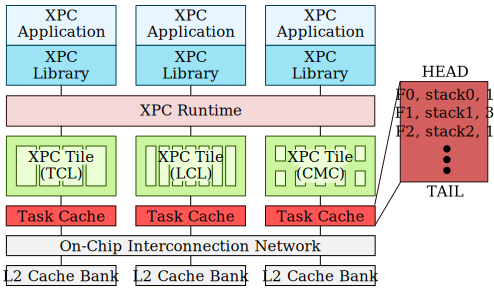
\includegraphics[width=\tw]{task-cache.svg.pdf}

  \caption{\textbf{Task Cache Diagram --} Per-core task caches store
    generated tasks in hardware as a triplet of a function pointer, a
    stack pointer, and the number of calls for the task.}

  \label{fig-xpc-task-cache}

%\end{figure}


  \end{minipage}%
  \hfill%
  \begin{minipage}[b]{0.45\tw}
    %=========================================================================
% fig-xpc-task-network.tex
%=========================================================================

%\begin{figure}

  \centering
  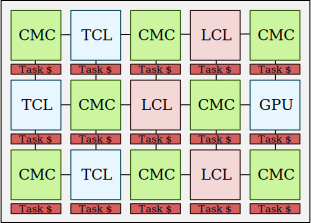
\includegraphics[width=\tw]{task-network.svg.pdf}

  \caption{\textbf{Task Distribution Network Diagram --} Network
    connecting task caches for rapid distribution of tasks across
    heterogeneous XPC tiles based on meta-data describing task affinity
    with given tile.}

  \label{fig-xpc-task-network}

%\end{figure}


  \end{minipage}
\end{figure}

To schedule fine-grain parallel tasks, an adaptive runtime is required to
dynamically match tasks with tiles optimal for the exhibited type of
parallelism. This process can be accelerated with a \emph{task cache} and
\emph{task distribution network} for storing and distributing tasks in
hardware.

The software runtime is responsible for managing the aforementioned
cactus stack as well as facilitating task stealing between threads or XPC
tiles based on heuristics collected to reflect how well suited the task
is for the given tile. A critical component to the task stealing in the
context of a heterogeneous architecture is determining key heuristics
for accurately predicting the optimal tile for executing a task. An
initial idea is the collect statistics on control and memory-access
irregularity to proxy performance and energy efficiency. Higher
irregularity would suggest the task is better suited for more
general-purpose tiles, whereas highly regular tasks would be better
suited for specialized accelerator tiles. Another idea would be to
utilize a profiling phase to run tasks on different tiles to determine
the highest performing tile for a given application.

The runtime normally generates and distributes tasks through memory, but
the XPC architecture can use hardware acceleration to streamline these
processes. Figure~\ref{fig-xpc-task-cache} shows a per-tile \emph{task
  cache} that exploits intra-tile task locality by storing generated
tasks in a hardware cache to avoid memory accesses. This is based on the
observation that each thread or tile will almost always need to access
its own cactus stack whenever it is ready to execute a new
task. Furthermore, Figure~\ref{fig-xpc-task-network} shows a \emph{task
  distribution network} connecting task caches to facilitate rapid
distribution of tasks to tiles attempting to steal tasks. The runtime
triggers a broadcast of task steal requests if the tile it is running on
is idle. For scalability, the request is only broadcasted to the tile's
direct neighbors. The network also communicates meta-data with each
request describing the type of task for which it is best suited, which
can considered along with collected heuristics to determine whether or
not a tile should allow task stealing. These hardware techniques for
storing and distributing tasks is inspired by our previous work in
improving load balancing on GPGPUs~\cite{kim-hwwl-micro2014}.

\subsection{Executing Fine-Grain Parallel Tasks}

To execute fine-grain parallel tasks, the techniques for exposing and
scheduling tasks detailed above can be applied to either a traditional
multicore microarchitecture or to a fine-grain heterogeneous mix of XPC
tiles specialized for varying levels of amorphous data parallelism.

Mapping to a traditional multicore microarchitecture allows legacy
systems to take advantage of the unified tools and cleanly exposed
parallelism offered by the XPC framework. However, this approach is
unable to fully tap into the potential for seamless adaptive execution of
tasks exhibiting varying forms of amorphous data parallelism.

In order to take advantage of the techniques for exposing and scheduling
fine-grain parallel tasks introduced by the XPC framework, a fine-grain
heterogeneous microarchitecture is required. Several XPC tiles, ranging
from highly specialized to general-purpose, are provided to allow dynamic
scheduling of tasks to the tile best suited for exploiting the associated
form of amorphous data parallelism.

\textbf{XPC Tightly-Coupled Lanes (TCL) --} The TCL XPC tile is a
highly-specialized accelerator for regular amorphous data parallelism. A
simple in-order, single-issue control processor is tightly coupled with a set
of computation lanes. Instruction fetch and decode are
amortized by the control processor then issued to an issue unit
which schedules a group of threads which execute in lock-step
(i.e., warps) on the tightly-coupled computation lanes. Control
irregularity can cause divergence between threads, serializing execution
of both paths of the branch. Memory accesses are dynamically coalesced by
a memory unit by comparing the addresses generated across the
lanes. Unlike GPGPUs, TCL focuses on exploiting intra-warp parallelism
instead of relying on extreme temporal multithreading to exploit
inter-warp parallelism. Due to its lightweight, embedded design, TCL is a
natural fit for the heterogeneous XPC architecture. The TCL design is
inspired by our previous work in area-efficient, embedded SIMT
architectures~\cite{kim-simt-vstruct-isca2013}, and similar techniques
can be used to eliminate redundant computation to further improve
performance and energy efficiency of regular amorphous data parallel
workloads.

Although we predict that TCL will achieve high performance and energy
efficiency by amortizing the front-end and memory accesses as well as
exploiting value structure for traditional data parallel applications, we
imagine that it will struggle with the serialization causes by control
and memory-access irregularity in more irregular amorphous data parallel
applications.

\textbf{XPC Loosely-Coupled Lanes (LCL) --} The LCL XPC tile is a
highly-specialized accelerator for slightly more irregular amorphous data
parallelism. The key difference between the TCL and LCL is that the LCL
allows for decoupling in control flow between lanes without significant
overheads. This is achieved by using per-lane instruction buffers which are
populated by the control processor and can contain different sections of
code for each lane to execute. The control processor still amortizes
instruction fetch, but issues coarser-grain tasks to the lane management
unit which efficiently distributes work across the lanes. Each LCL lane
is more lightweight than the TCL counterpart as it shares expensive
long-latency functional units between all lanes and the control
processor. This allows us to employ more LCL lanes than TCL lanes for
roughly the same cost. The LCL design is inspired by previous work on
accelerating loop patterns in hardware~\cite{srinath-xloops-micro2014}.

We envision LCL to be a reasonable middle-ground between the TCL and CMC
tiles (discussed below) because although it has a higher tolerance for
control irregularity, LCL is still better suited for simpler tasks on the
lanes and can suffer from high memory-access irregularity.

\textbf{XPC Cooperative Multicore (CMC) --} The CMC XPC tile is a
general-purpose multicore processor designed to be used for highly
irregular amorphous data parallel applications. A grid of discrete cores
are connected by a mesh network to facilitate inter-core
communication. Each CMC core, albeit relatively simple, is akin to a
stripped-down control processor in a TCL/LCL tile, making it capable of
handling high control and memory-access irregularity with acceptable
performance. The tradeoff is that CMC is the least energy efficient tile
of the three XPC tiles for applications which do not exhibit highly
irregular amorphous data parallelism. They key difference between the CMC
tile and a traditional multicore is that the CMC tile uses hardware
acceleration for scheduling fine-grain parallel tasks as described above,
both at the intra-tile and inter-tile levels.

The CMC tile could function as a default tile for the profiling phase
when statistics are collected to determine if a specialized tile would be
more suitable, in addition to being the optimal tile for highly irregular
amorphous data parallel applications which cannot fully utilize the
amortization offered by the TCL or LCL.

